\documentclass[letter,10pt]{article}
\usepackage{authblk}
\usepackage{geometry}
\geometry{margin=1.0in}
\usepackage{graphicx}
\graphicspath{ {./images/} }
\usepackage{enumitem}
\usepackage{amsmath}
\usepackage{amssymb}
\usepackage{biblatex}
%\usepackage[backend=biber]{biblatex}
\addbibresource{references.bib}

\begin{document}
\title{The Hollow Heap Data Structure: An Introduction, Run-Time Analysis, and Comparison to the Fibonacci Heap}
\author{Alisha Sprinkle and Courtney Dixon}
%\affil{CS 5110 - The Design and Analysis of Algorithms}
\date{December 8, 2019}
\maketitle

\section{Abstract}
\quad Hollow Heaps were introduced by Hansen, Kaplan, Tarjan, and Zwick in 2015. This data structure performs operations with the same amortized efficiency as the Fibonacci Heap introduced by Tarjan and Fredman. Hollow Heaps perform all operations characteristic of a heap, however, Hollow Heaps use lazy deletion and a directed acyclic graph rather than trees. The goal of this paper is to explain the Hollow Heap data structure precisely, analyze the amortized running time of the data structure, implement the data structure in Java, and compare the efficiency of Hollow Heaps to the renown Fibonacci Heap data structure.

\section{Hollow Heaps}
\quad A Hollow Heap is a heap-ordered data structure. Therefore, a Hollow Heap maintains the heap property; the key of Node a is less than or equal to the key of Node b for every directed arc(a,b) in the structure where Node a is the parent of Node b. The typical properties of nodes still hold as well. A root is a node that does not have a parent and a leaf is a node that does not have any children. The root of a Hollow Heap has the minimum key in the Hollow Heap.\\

Hollow Heaps are just as efficient as Fibonacci Heaps. All the operations of a heap, excluding two, take $O(1)$ time in the worst case and amortized with Hollow Heaps. The two heap operations that take longer than constant time are \textit{delete} and \textit{deleteMin}, which each take $O(\log n)$ amortized time with Hollow Heaps. The \textit{decreaseKey} operation in Hollow Heaps uses lazy deletion and reinsertion. Using lazy deletion prevents cascading cuts and this separates Hollow Heaps from Fibonacci Heaps. Other heaps use a tree or set of trees, but Hollow Heaps use a directed acyclic graph (dag) instead.\\

A Hollow Heap is made up of nodes that hold items and not the typical nodes that are items. HollowNodes have two integer fields, one Node field, and three HollowNode fields. The two integers are key and rank. The key is the value that the item in the HollowNode holds. The rank is the rank of the HollowNode in the HollowHeap. The Node field points to the item that the HollowNode is holding. The three HollowNode fields are child, next, and extra parent. The child field points to the last child of the HollowNode. As a HollowNode gains children they are put at the beginning of the list of children. The next field points to the sibling of the HollowNode. This allows us to traverse the list of children belonging to a HollowNode. The extra parent field points to a HollowNode that is the second parent of the HollowNode pointing to it. A second parent is gained when a HollowNode becomes hollow when the item it is holding is deleted or the key has been decreased causing the item to be stored in a new HollowNode entirely. The item that the HollowNode is holding is of type Node. The Node type has two fields. One integer field to hold the key and one HollowNode field that points to the HollowNode that is holding the item. The node structures are depicted in the image below.\\
\begin{center}
	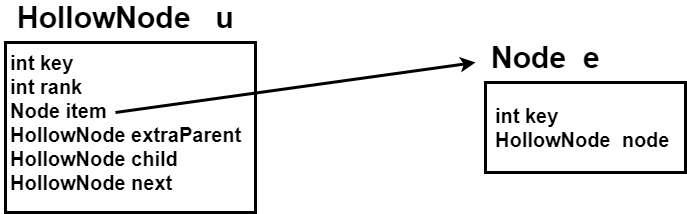
\includegraphics[scale=.5]{one.png}\\
	\phantom{helloworld}
	HollowNode u holds an item, Node e.\\
	Node e has a reference to HollowNode u\\
\end{center}

\medskip

\section{Hollow Heap Implementation} 
\quad The authors presented three variants of the Hollow Heap data structure: Multi-Root, One-Root, and Two-Parent. The focus of this paper is the Two-Parent Hollow Heap; the final Hollow Heap data structure presented in the original paper. The Two-Parent Hollow Heap uses a directed acyclic graph (dag) that rids the algorithm of having to move children. The Two-Parent Hollow Heap performs the classic heap operations: \textit{makeHeap}, \textit{findMin}, \textit{insert}, \textit{deleteMin}, \textit{meld}, \textit{decreaseKey}, and \textit{delete}.\\ 

\quad The \textit{makeHeap} method returns a new Hollow Heap that is empty. The \textit{findMin} method returns the item pointed to by the minimum HollowNode in the Hollow Heap. The \textit{insert} method returns a new Hollow Heap that contains all the old elements of the original Hollow Heap and the new element that was to be inserted. The \textit{deleteMin} method removes the minimum element from the Hollow Heap. The \textit{meld} method takes two Hollow Heaps and returns a Hollow Heap that is the combination of the two original Hollow Heaps. The \textit{decreaseKey} method changes the key of the element to the provided key. A call to \textit{decreaseKey} makes an entirely new HollowNode with a new Node both with the new key and the old HollowNode is made hollow. The \textit{delete} method removes an element.\\ 

\quad In addition to the classic heap methods, the Two-Parent Hollow Heap also has the following methods: \textit{makeNode}, \textit{link}, \textit{addChild}, \textit{doRankedLinks}, \textit{doUnrankedLinks}. The \textit{makeNode} method takes an item of type node and an integer key and makes a new HollowNode that holds the Node item with the key specified. When a new HollowNode is created it is considered full.  A HollowNode becomes hollow after a call to \textit{decreaseKey} or a call to \textit{delete}. A HollowNode can never become full again and remains hollow until it is destroyed. The \textit{link} method takes two HollowNodes and determines which one has the smaller key. The HollowNode with the smaller key becomes the parent of the HollowNode whose key is larger. The paper calls the parent HollowNode the ``winner" and the child HollowNode the ``loser". The \textit{link} method returns the parent HollowNode, the ``winner". The \textit{addChild} method takes two HollowNodes and makes the first the sibling of the child of the second. The \textit{doRankedLinks} method is used by the \textit{delete} method and calls the \textit{link} method based on the ranks of the HollowNodes in the HollowHeap. The \textit{doUnrankedLinks} method is also used by the \textit{delete} method and calls the \textit{link} method regardless of the ranks of the HollowNodes in the HollowHeap. 

\section{Amortized Analysis via the Accounting Method}
The \textit{insert} operation is responsible for the creation of HollowNodes and therefore will be overcharged by $O(1)$ to account for the future \textit{decreaseKey} operation that results in a rebuilding of the Hollow Heap. The rebuilding occurs when the number of \textit{insert} operations plus the number of \textit{decreaseKey} operations exceeds the number of full nodes multiplied by a constant greater than one. In formulaic form, rebuilding occurs when $N > cn: c > 1$, where $N$ is the number of \textit{insert} operations plus the number of \textit{decreaseKey} operations, $n$ is the number of full HollowNodes in the Hollow Heap, and c is a constant larger than one that makes the algorithm most efficient for some $n$ sized Hollow Heap \cite{hollow}. The same formula is true for a rebuild triggered by a call to the \textit{delete} method.\\

For the \textit{decreaseKey} and \textit{delete} results in the chart below, we will assume 17 \textit{insert} operations have already occurred and our $c = 2$. The two charts are the same because \textit{decreaseKey}, \textit{delete}, and \textit{deleteMin} all use some form of lazy deletion. The \textit{decreaseKey} method makes a new HollowNode with the new key and makes the old HollowNode hollow instead of getting rid of it to prevent moving children. The \textit{deleteMin} method calls the \textit{delete} method, so the analysis is treated the same. The \textit{delete} method just makes HollowNode hollow instead of getting rid of it to also prevent moving children. The \textit{decreaseKey} and \textit{delete} methods each take $O(\log n)$ amortized time because of the potential of a rebuilding that traverses the entire dag of height $O(\log n)$ getting rid of HollowNodes and linking full HollowNodes possibly using ranks depending on the event that triggered the rebuild.\\
\begin{center}
	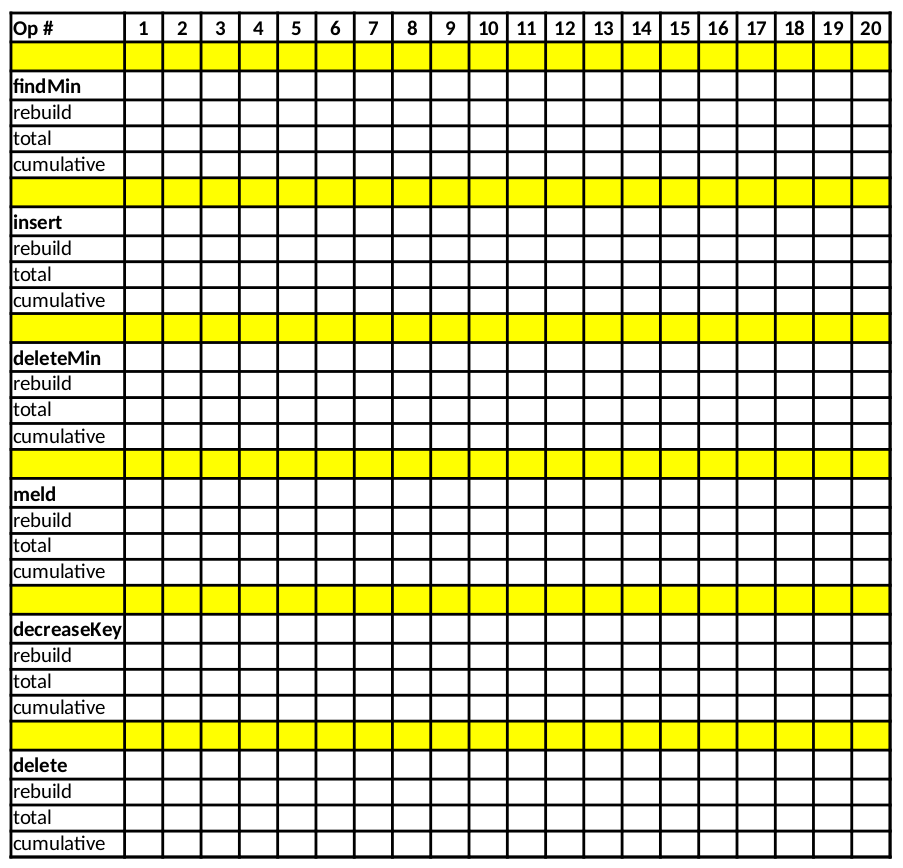
\includegraphics[width=\textwidth]{accounting.png}
\end{center}

\section{Hollow versus Fibonacci: A Comparison}
\quad Our implementation is of the Two-Parent Hollow Heap. We implemented the classic Fibonacci Heap so that we could compare the two data structures in terms of practical efficiency. Our programs are written in the Java programming language. Our source code can be found at \textit {https://github.com/dixoncs/CS5110-Fall2019.git}. The following UML diagrams are for our HollowHeap and FibonacciHeap classes. 
\begin{center}
	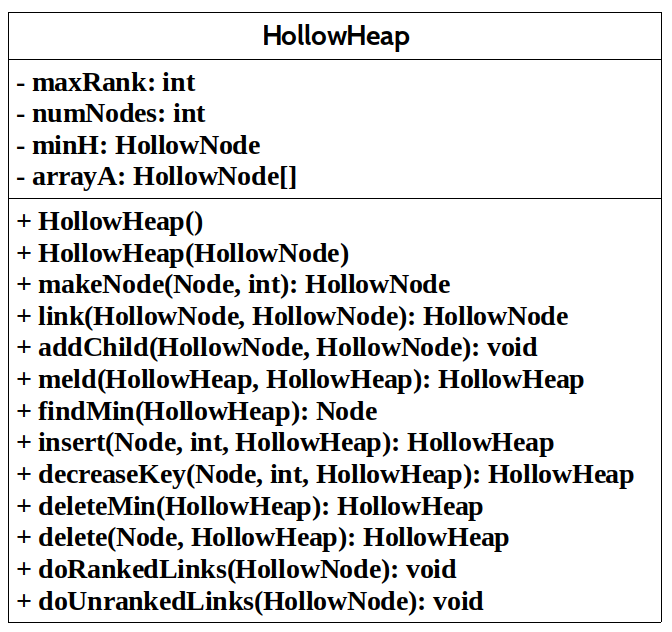
\includegraphics[scale=0.32]{hollowuml.png}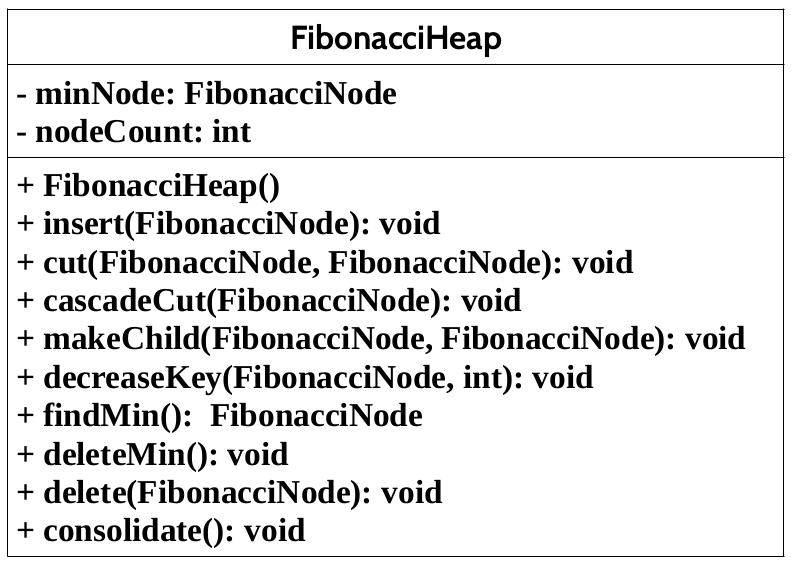
\includegraphics[scale=0.32]{fibonacciheapuml.png}
\end{center}
\quad As you can see in the diagrams above, the methods for the two implementations are quite different. The Fibonacci Heap handles cascading cuts whereas the Hollow Heap avoids these cuts by using HollowNodes and lazy deletion. The Fibonacci Heap methods almost all have a void return type, but the Hollow Heap methods return either a Hollow Heap or a HollowNode. This difference lead to some creativity in method calls. There are differences in the node structures as well. The FibonacciNode has four pointers to keep track of the parent, child, left, and right FibonacciNodes as well as two integer fields and a boolean member. The first integer is for the key, the second is for the degree, and the boolean is to keep track of marked-ness. The HollowNode also has four pointers to node structures but only three are of type HollowNode. The item field is a pointer to a Node data type. There is still an integer type for the key and a rank fields which is consistent with the Fibonacci Heap fields. The Hollow Heap has a couple more methods than the Fibonacci Heap and this is because of the difference in the rebuilding process. Two-Parent Hollow Heaps are represented as a directed acyclic graph instead of a tree or set of trees like the Fibonacci Heap. Fibonacci Heaps and Hollow Heaps both have the same amortized runtime analysis. All of the classic heap methods run in $O(1)$ amortized time except \textit{decreaseKey} and \textit{delete}, which run in $O(\log n)$ amortized time for a $n$ element heap of height $O(\log n)$. The two heap types are both supposedly simple to implement. 

\section{Conclusion}
Hollow Heaps are directed acyclic graphs that use lazy deletion and reinsertion to avoid cascading cuts and having to move children. Hollow Heaps use a HollowNode data structure that holds an item of a Node data type. Hollow Heaps have all the classic heap methods and these methods run in the same amortized time as the same methods in Fibonacci Heaps. We did not find a significant difference between Fibonacci Heaps and Hollow Heaps through side by side programmatic testing. In the future we would like to complete the implementation of Hollow Heaps so that we can run more extensive tests with larger data sets to determine if Hollow Heaps are in fact an improvement of Fibonacci Heaps as claimed by the authors. 

\section{Figures}

\medskip
\phantom{helloworld}
\begin{center}
	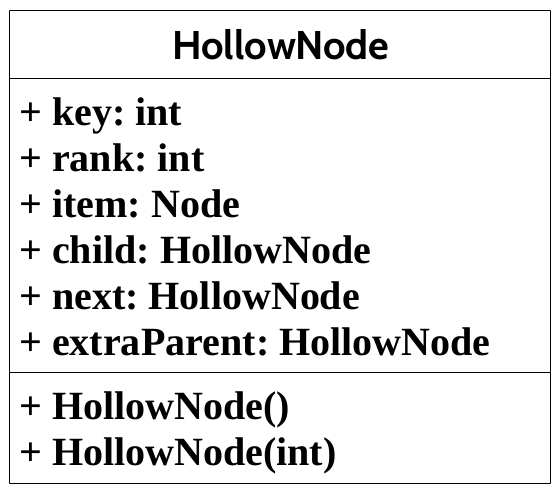
\includegraphics[scale=.32]{hollownodeuml.png} \phantom{helloworld}	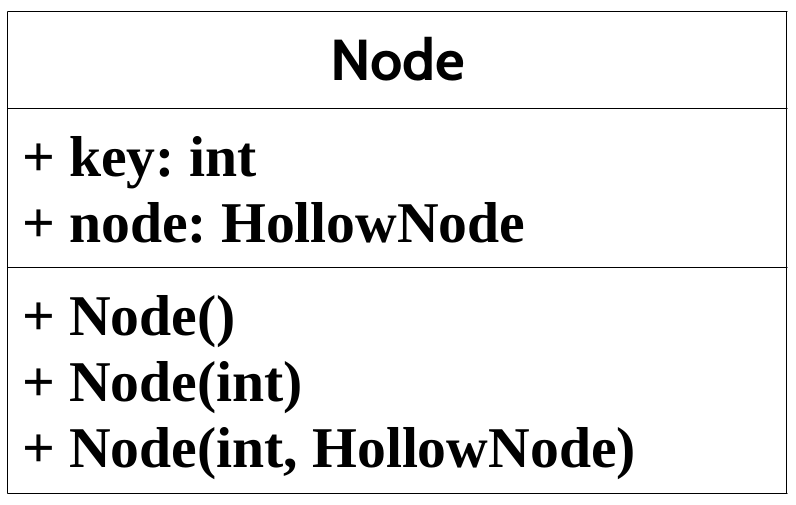
\includegraphics[scale=.24]{nodeuml.png}\\
\end{center}
\qquad \qquad HollowNode Class UML Diagram \phantom{helllloooooowoooorld} Node Class UML Diagram

\medskip

\begin{center}
	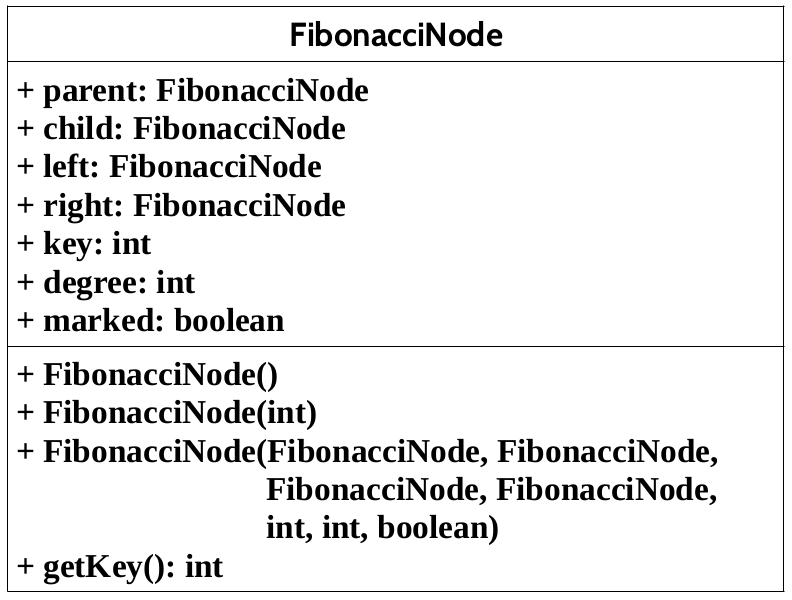
\includegraphics[scale=.32]{fibonaccinode.png}\\
	FibonacciNode Class UML Diagram
\end{center}

\medskip

%\begin{center}
%	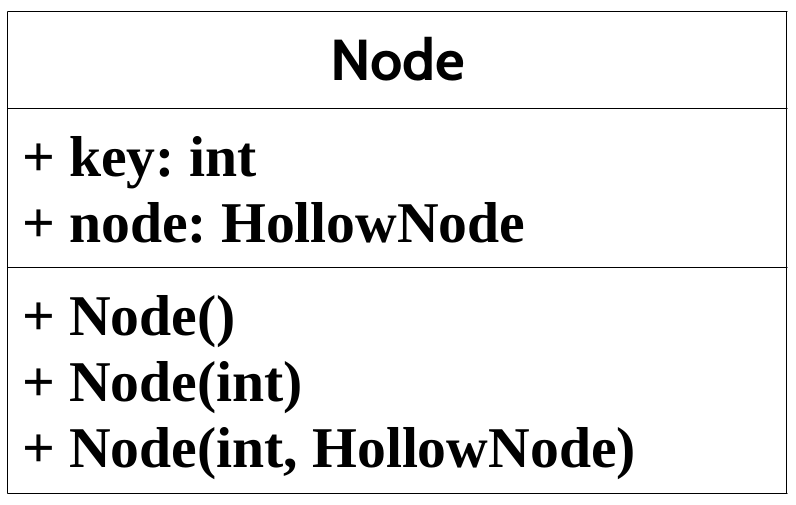
\includegraphics[scale=.24]{nodeuml.png}\\
%	Node Class UML Diagram
%\end{center}

\medskip

\begin{center}
	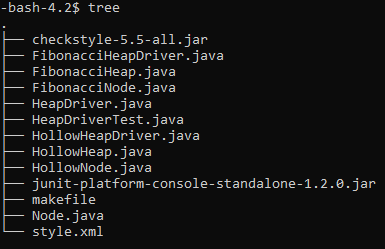
\includegraphics[]{tree.png}\\
	Directory Tree
\end{center}

\medskip

\begin{center}
	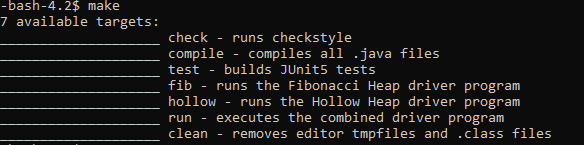
\includegraphics[]{make.png}\\
	Makefile Targets
\end{center}
%\begin{center}
%	\includegraphics[]{.png}
%\end{center}

\newpage
\nocite{*}
\printbibliography

\end{document}

